From chapter 2, we observe that a number of techniques have been studied for optimizing the performance of the PageRank algorithm. This is important, since one of the most important applications of PageRank, that is the ordering of search results on the web for a given query, requires operating on massive-scale graphs. Considering the fact that these graphs are constantly being updated, a number of techniques for dynamic PageRank computation have been developed. To date, powerful shared memory systems have achieved the best performance. This is thanks to the availability of multicore servers with more than a terabyte of memory, which can fit graphs with hundreds of billions of edges. These shared-memory multicores are significantly more efficient on time and energy basis, when compared to when compared to distributed memory systems \cite{graph-shun13}. In order to cope with low memory systems, streaming PageRank techniques have been developed which do not require storing the entire graph in memory for the computation \cite{pr-sarma11}.

% However, we find that most studies focus only on the teleport-based dead end handling strategy for PageRank, as recommended by the Original Google patent. Thus, algorithmic optimization techniques that could be applied to other dead end handling strategies were left behind. Through our experimentation, we observe that teleport-based PageRank has the lowest performance among three other strategies.
The paper on STIC-D based algorithmic techniques for PageRank \cite{pr-sticd16} utilizes the decomposability of graphs. It allows for greater parallelization, given its lack of per-iteration communication requirement. It also serves as a good foundation for exact streaming PageRank since only a subset of the needs to be processed at a time. Given the demand for PageRank computation across disciplines, a study focused on the design of GPU-based implementation of the algorithm is essential.

% We also noted issues with performance comparison between the technique developed, and the state of the art in a few papers. This was because of the difference in choice of error measurement function, and measurement of time taken for computation, among other things. Average speedup in some cases was obtained by finding the speedup of the developed technique for each test case, and averaging them. The standard approach in the domain of bench-marking involves the use of geometric mean (GM). Thus, we find a detailed study of the effects of variations on the performance of PageRank to be essential before the development of a new optimization technique. This would help us pin down the factors that allow a certain technique to perform better than others.

Our initial focus is on collecting data on the effects of adjusting PageRank parameters, error measurement functions, and dead end handling strategies, and rank adjustment strategies. We develop a CUDA-based PageRank to act as a baseline for future PageRank techniques on the GPU.
The design of STIC-D based algorithmic techniques for PageRank \cite{pr-sticd16} involves both monolithic (non-decomposed) and levelwise (decomposed) versions. This helps with determining the factors that contribute to performance improvement. We expect that this analysis would in turn help with development of any further techniques or optimizations. Since some optimization techniques only work for a specific category of graphs, we wish to automatically determine the choice of using an optimization. Further study involves applying the developed techniques to streaming PageRank on the GPU.

% Individual repositories for each specific experiment would be maintained. This is in order to enable easy peer-review, as well as enabling other people easily verify the results for themselves. Additional helper packages would be written as per requirement. Integrations with existing graph frameworks may be done, if time permits.
% We have studied the effects of adjusting various aspects of the PageRank algorithm, and developed two suitable approaches for dynamic PageRank computation on the CPU, as well as the GPU. We hope this would be a stepping stone for us in developing suitable dynamic and streaming algorithms for massive real-world graphs.




% \section{PageRank Algorithm}

We first attempt to parallelize PageRank for the NVIDIA Volta GPU. The first step of our parallelization process is to independently parallelize map and reduce-like operations within the algorithm, to obtain a suitable implementation and launch config. The second step involves parallelizing the rank computation process using a \emph{switched thread/block-per-vertex} approach after the vertices have been partitioned by in-degree at a suitable switch point, and with apt launch configs for each partition. We observe that the sequential CPU-based vector element sum with 32-bit floating point values suffers from precision issues, while the CUDA-based does not.
% We first attempt to parallelize PageRank for the NVIDIA Volta GPU. GPUs are usually optimized for \emph{chunked memory access patterns} and \emph{high compute}. While the PageRank algorithm has an \emph{unchunked-gather memory access pattern} and \emph{low compute}, implementing it on a CUDA-enabled GPU, such as the Volta GV100, can bring a significant performance improvement. The first step of our parallelization process is to independently parallelize map and reduce-like operations within the algorithm, to obtain a suitable implementation and launch config. The second step involves parallelizing the rank computation process using a \emph{switched thread/block-per-vertex} approach after the vertices have been partitioned by in-degree at a suitable switch point, and with apt launch configs for each partition.
% Compared to nvGraph PageRank on fixed and temporal graphs, we observe a small performance improvement. We should however note that the CUDA implementation we develop here uses L1-norm for error measurement, while nvGraph PageRank uses L2-norm for error measurement, along with a per iteration L2-norm rank scaling followed by an L1-norm rank scaling after the final iteration. We should also remark that the sequential CPU-based vector element sum with 32-bit floating point values suffers from precision issues, while the CUDA-based does not.

% \begin{figure*}[!hbtp]
  \centering

  \subfloat{
    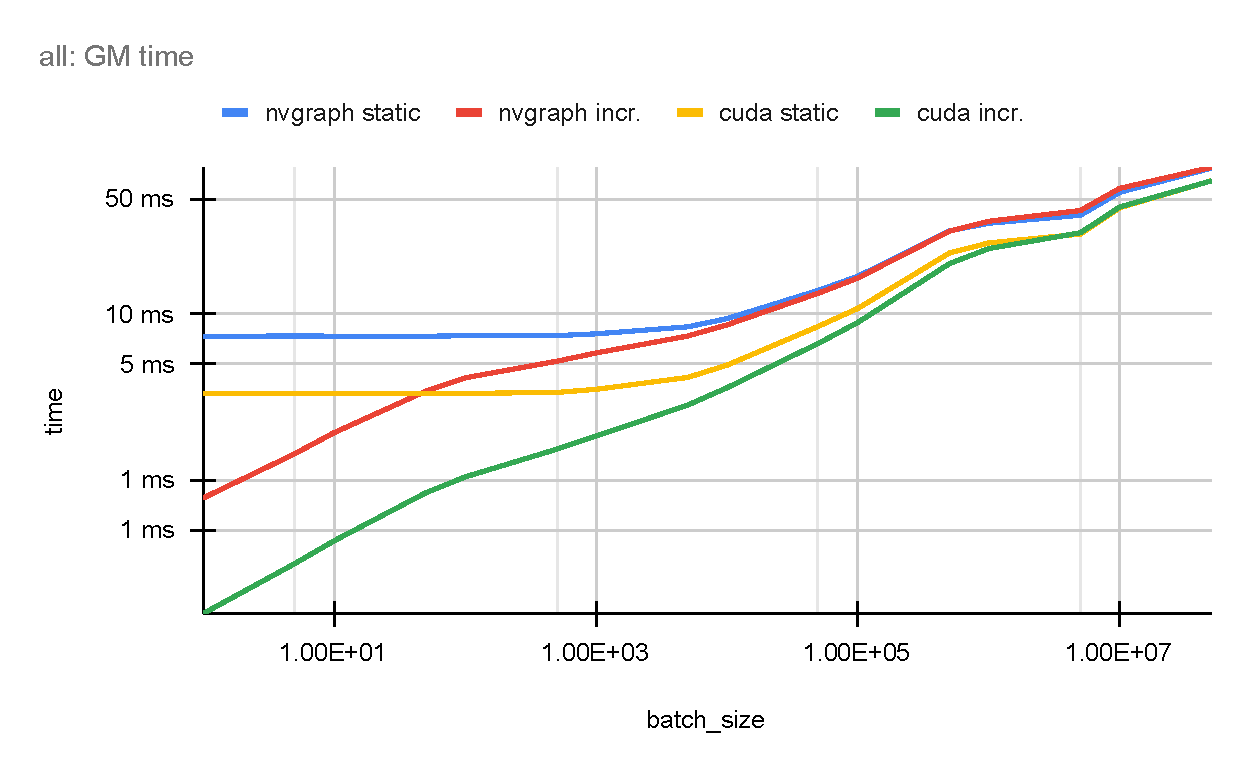
\includegraphics[width=0.48\textwidth]{out/pr-cuda-st-vs-it-time.pdf}
    \label{fig:pr-cuda-st-vs-it-time}
  }
  \subfloat{
    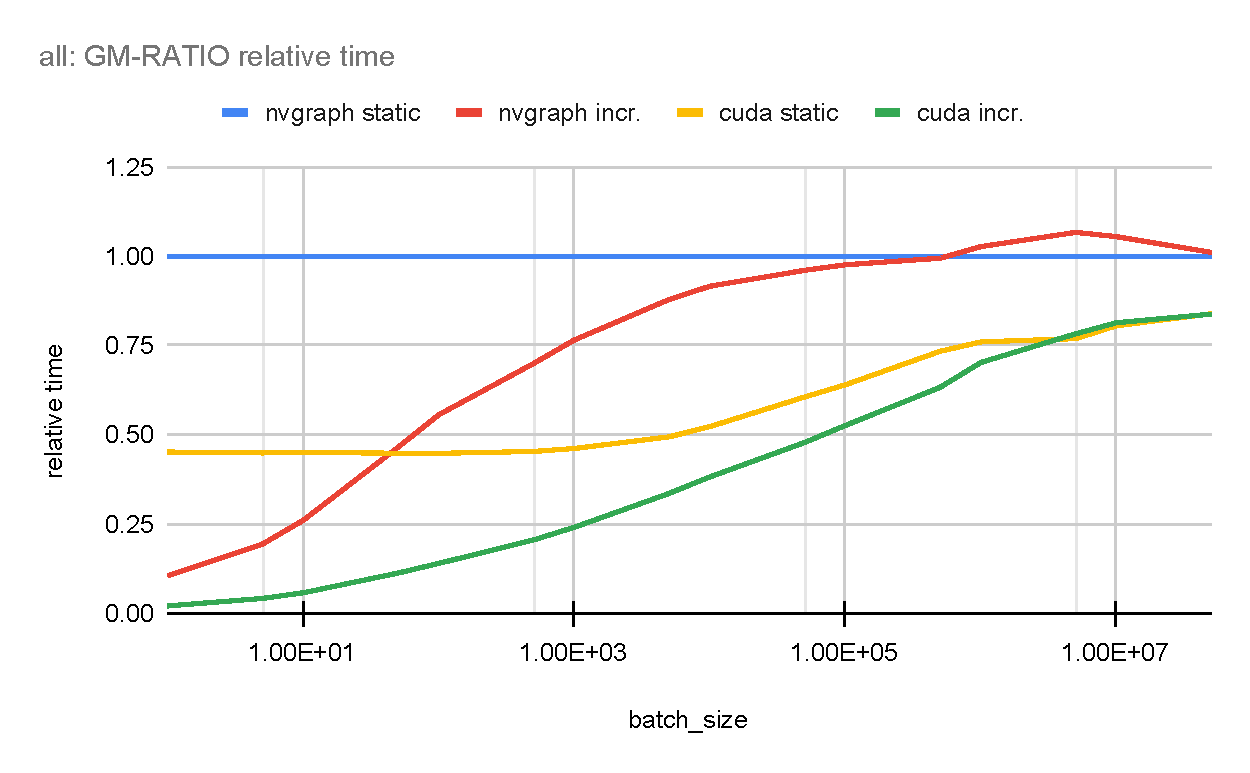
\includegraphics[width=0.48\textwidth]{out/pr-cuda-st-vs-it-rtime.pdf}
    \label{fig:pr-cuda-st-vs-it-rtime}
  }

  \caption{GM time taken for static and incremental PageRank with nvGraph and CUDA implementation, with respect to nvGraph’s static PageRank is shown on the left. Relative GM time taken is shown on the right. This is done on seven temporal graphs. Error measurement between the previous and current iteration is done using L1-norm except for nvGraph, which uses L2-norm instead. Batch sizes range from $10^0$ to $5 * 10^7$.}
  \label{fig:pr-cuda-st-vs-it}
\end{figure*}



We then look into the effect on PageRank computation time for different datatypes of the rank vector and the CSR representation of graphs on both a CPU as well as a GPU. Results indicate that using a wider datatype for the CSR representation has a smaller impact to performance compared to using a wider datatype for the rank vector. This can be explained from the fact that the PageRank algorithm accesses the CSR representation in a linear-like fashion, which improves the cache hit ratio for a CPU, and improves memory coalescing for a GPU. On the other hand, it accesses the rank vector in random order. When a wider datatype is used, a higher memory bandwidth is required, and if memory accesses are random, cache memory can get occupied faster and require faster evictions, slowing down performance. In all cases however, the impact on performance for a wider datatype is higher for GPU, compared to CPU. This is likely because of architectural differences between the two devices, with the GPU having a wider memory bus than the CPU.
% We then look into the effect on PageRank computation time for different datatypes of the rank vector and the CSR representation of graphs. We try this on both a CPU, as well as a GPU. Results indicate that using a wider datatype for the CSR representation has a smaller impact to performance compared to using a wider datatype for the rank vector. This is despite the fact that the CSR representation has a much larger memory footprint, and thus higher memory access requirement, than the rank vector. This can be explained from the fact that the PageRank algorithm accesses the CSR representation in a linear-like fashion, which improves the cache hit ratio for a CPU, and improves memory coalescing for a GPU.
% On the other hand, it accesses the rank vector in random order. When a wider datatype is used, a higher memory bandwidth is required, and if memory accesses are random, cache memory can get occupied faster and require faster evictions, slowing down performance. In all cases however, the impact on performance for a wider datatype is higher for GPU, compared to CPU. This is likely because of architectural differences between the two devices, with the GPU having a wider memory bus than the CPU.

% \begin{figure*}[!hbtp]
  \centering

  \subfloat{
    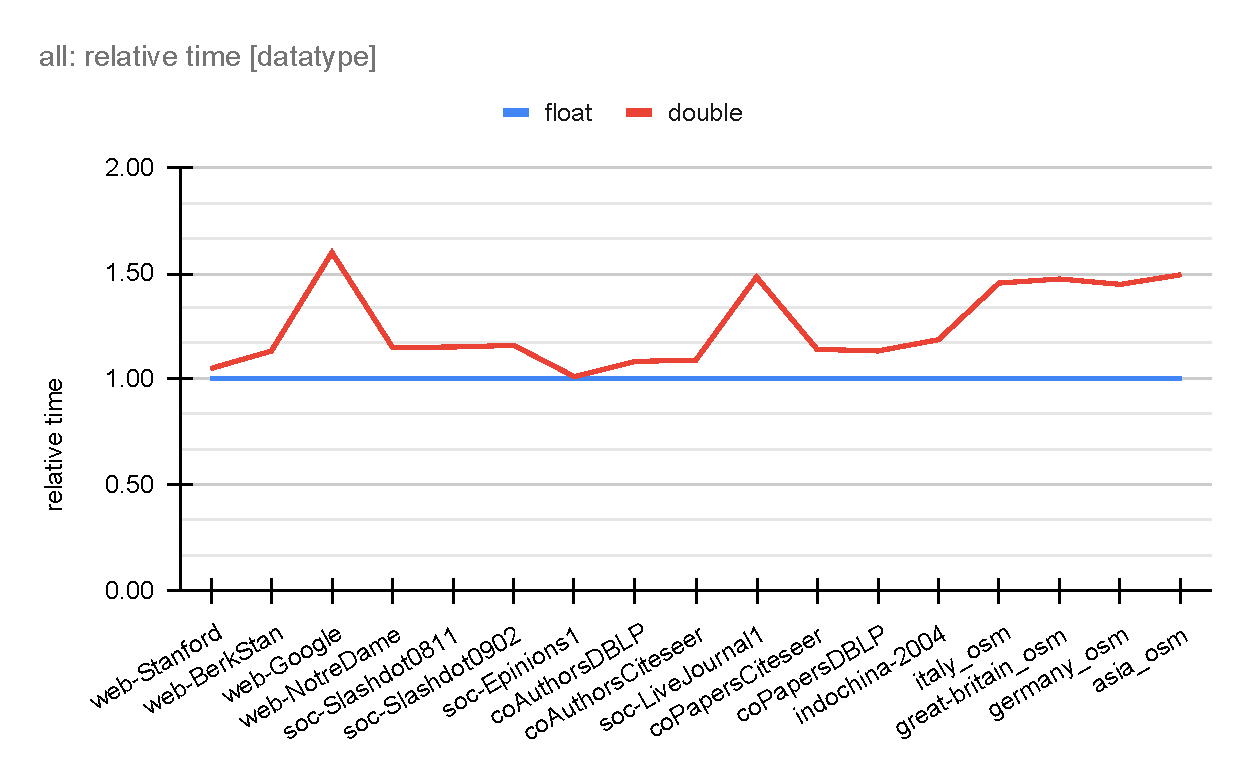
\includegraphics[width=0.48\textwidth]{out/pr-cuda-adj-rtype-rtime.pdf}
    \label{fig:pr-cuda-adj-rtype-rtime}
  }
  \subfloat{
    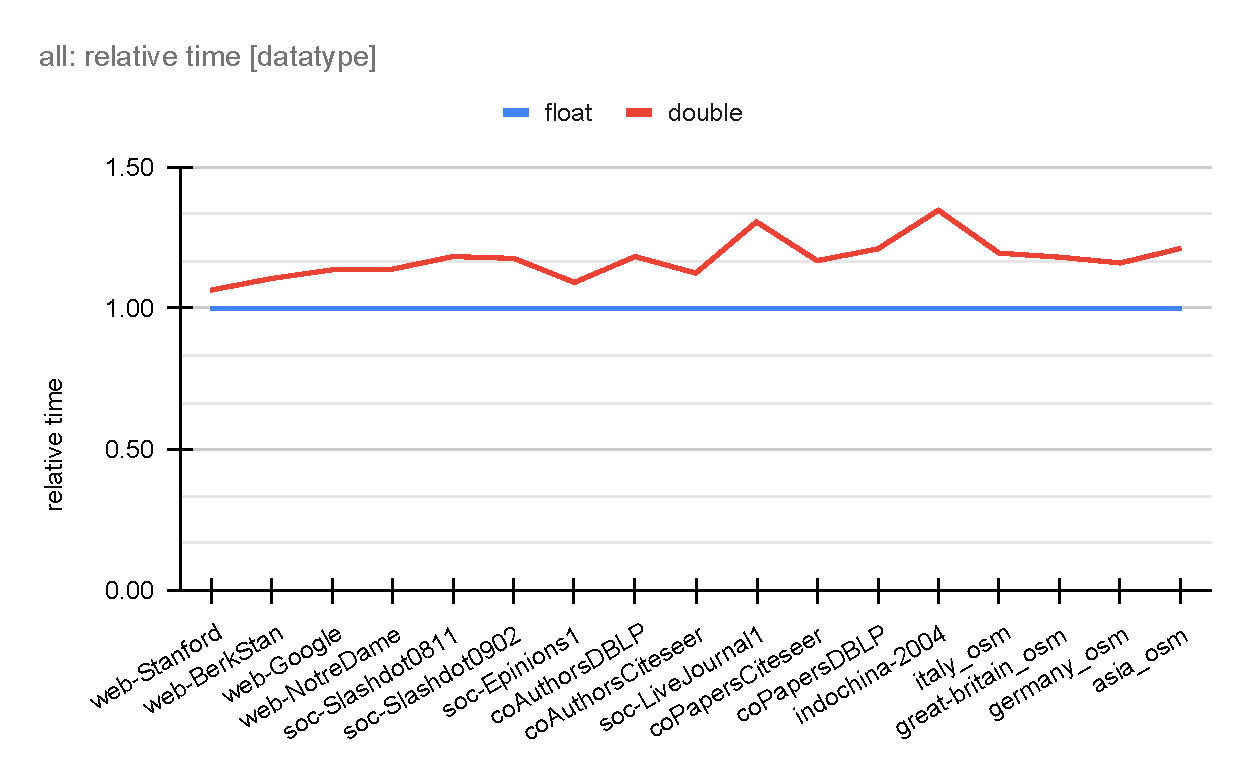
\includegraphics[width=0.48\textwidth]{out/pr-cuda-adj-ctype-rtime.pdf}
    \label{fig:pr-cuda-adj-ctype-rtime}
  }

  \caption{Relative time taken for switched thread/block-per-vertex CUDA-based (GPU) PageRank computation with the following datatypes for the rank vector is shown on the left: 32-bit floating point (float), 64-bit floating point (double). Relative time taken for CSR representation with the following datatypes is shown on the right: 32-bit integer (int32), 64-bit integer (int64). This is done on 5 web graphs, 4 social networks, 4 collaboration networks, and 4 road networks.}
  \label{fig:pr-cuda-adj-type}
\end{figure*}



We then explore the performance benefits of five different algorithmic optimizations for PageRank as presented in STIC-D paper \cite{pr-sticd16}, but without splitting the computation of ranks into multiple levels. The first two include splitting vertices by components, and sorting components by topological order in block-graph. The remaining three optimizations include skipping computation on in-identical, chain, and converged vertices. Again, we do this on both a CPU, as well as a GPU.
Our results indicate that splitting vertices by components provides a small performance improvement on average on both the devices. However, sorting components provides little additional benefit. The other three optimizations are beneficial only on certain graphs, but are detrimental on others due to their associated cost. Therefore, skip in-identical and chain optimizations should be applied only on graphs with a large number of in-identical and chain vertices respectively. In contrast, as the applicability of skip converged optimization cannot be predicted beforehand, it can be ignored. Moreover, in all cases the impact on performance is lower for GPU, compared to CPU. This is possibly because of the warp divergence introduced by the three skip optimizations due to irregular skipping of rank computation of vertices.

% \begin{figure*}[!hbtp]
  \centering

  \subfloat{
    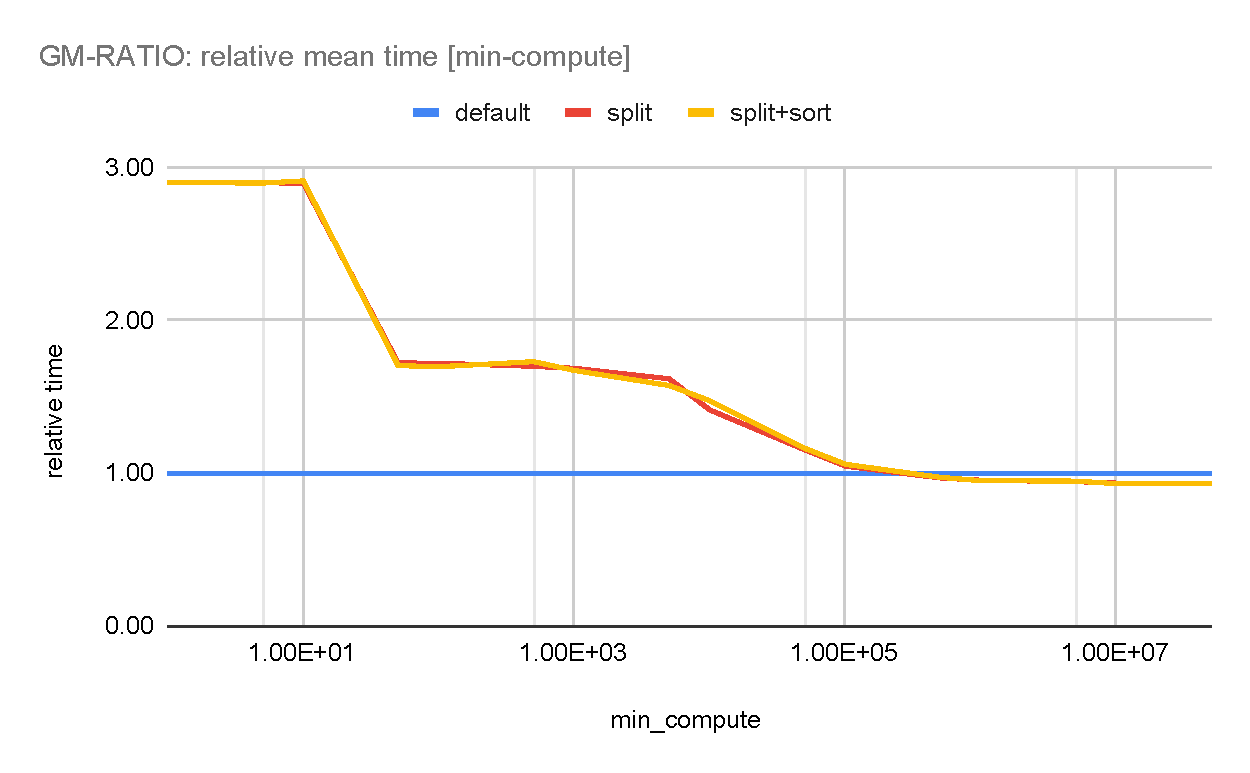
\includegraphics[width=0.48\textwidth]{out/pr-cuda-opt-s-rtime.pdf}
    \label{fig:pr-cuda-opt-s-rtime}
  }
  \subfloat{
    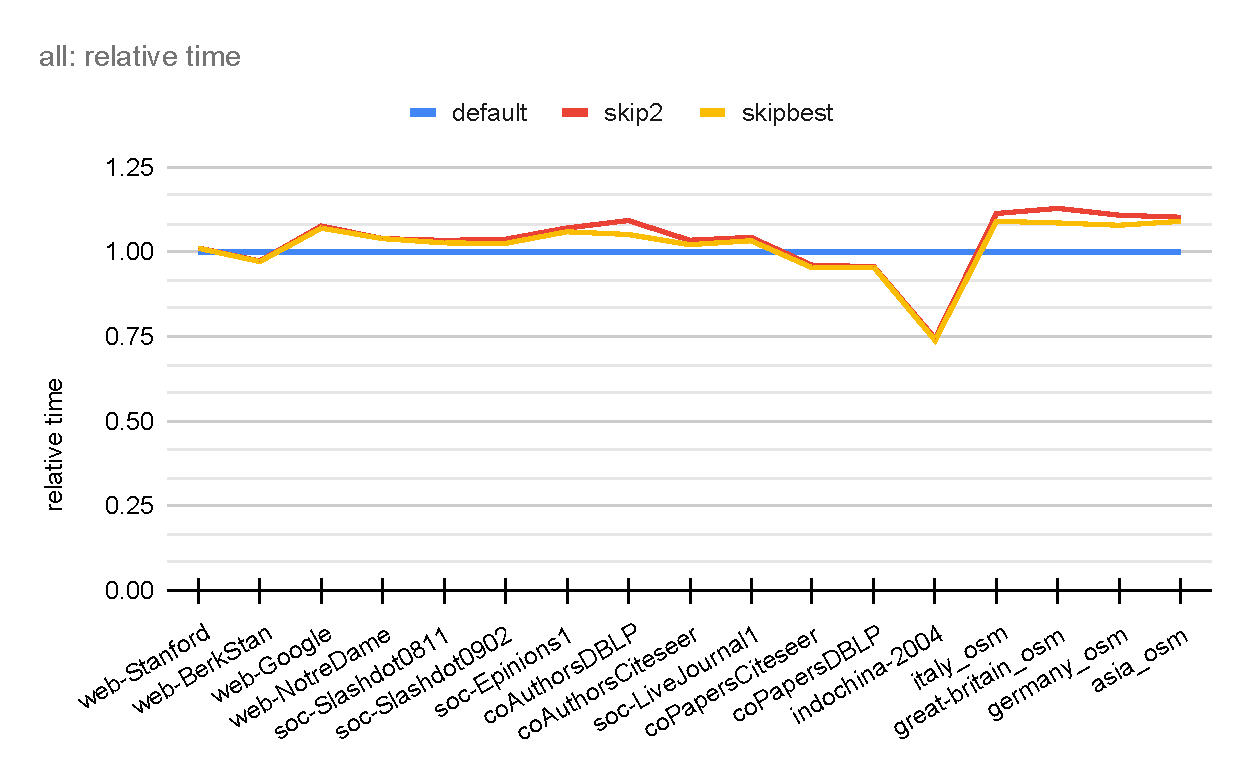
\includegraphics[width=0.48\textwidth]{out/pr-cuda-opt-i-rtime.pdf}
    \label{fig:pr-cuda-opt-i-rtime}
  }

  \caption{\textbf{Left:} Relative GM of time taken on all graphs for switched thread/block-per-vertex CUDA-based (GPU) static PageRank computation with the following algorithmic optimizations: no optimization (default), split vertices by components (split), and split vertices by components with each component sorted in topological order of its block-graph  (split+sort). This is relative to no optimization, with min. compute size ranging from 1 to 5×107. \textbf{Right:} Rel. time taken for switched thread/block-per-vertex CUDA-based (GPU) static PageRank computation with the following algorithmic optimizations: no optimization (default), skip all in-identicals (skip2), and skip in-identicals of best min. size  (skipbest). The ratio is obtained with respect to no optimization. This is done on 5 web graphs, 4 social networks, 4 collaboration networks, and 4 road networks.}
  \label{fig:pr-cuda-opt-si}
\end{figure*}

% \begin{figure*}[!hbtp]
  \centering

  \subfloat{
    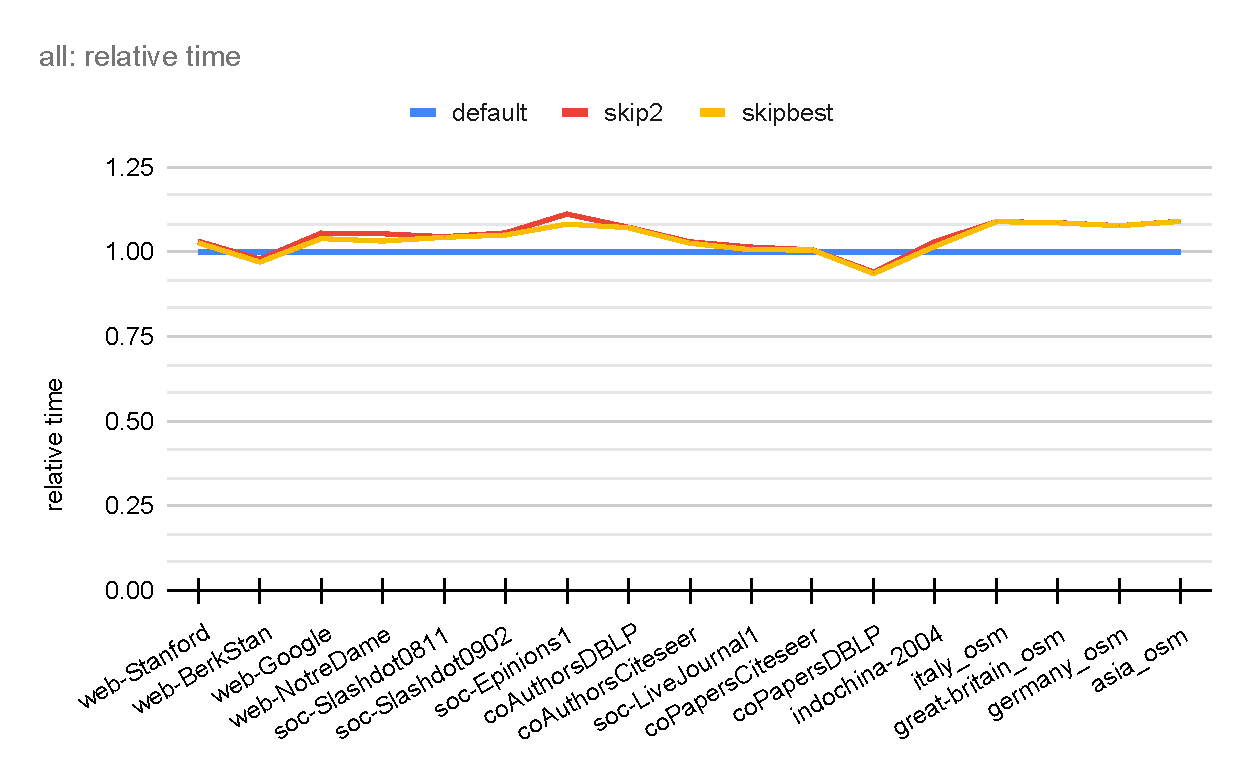
\includegraphics[width=0.48\textwidth]{out/pr-cuda-opt-c-rtime.pdf}
    \label{fig:pr-cuda-opt-c-rtime}
  }
  \subfloat{
    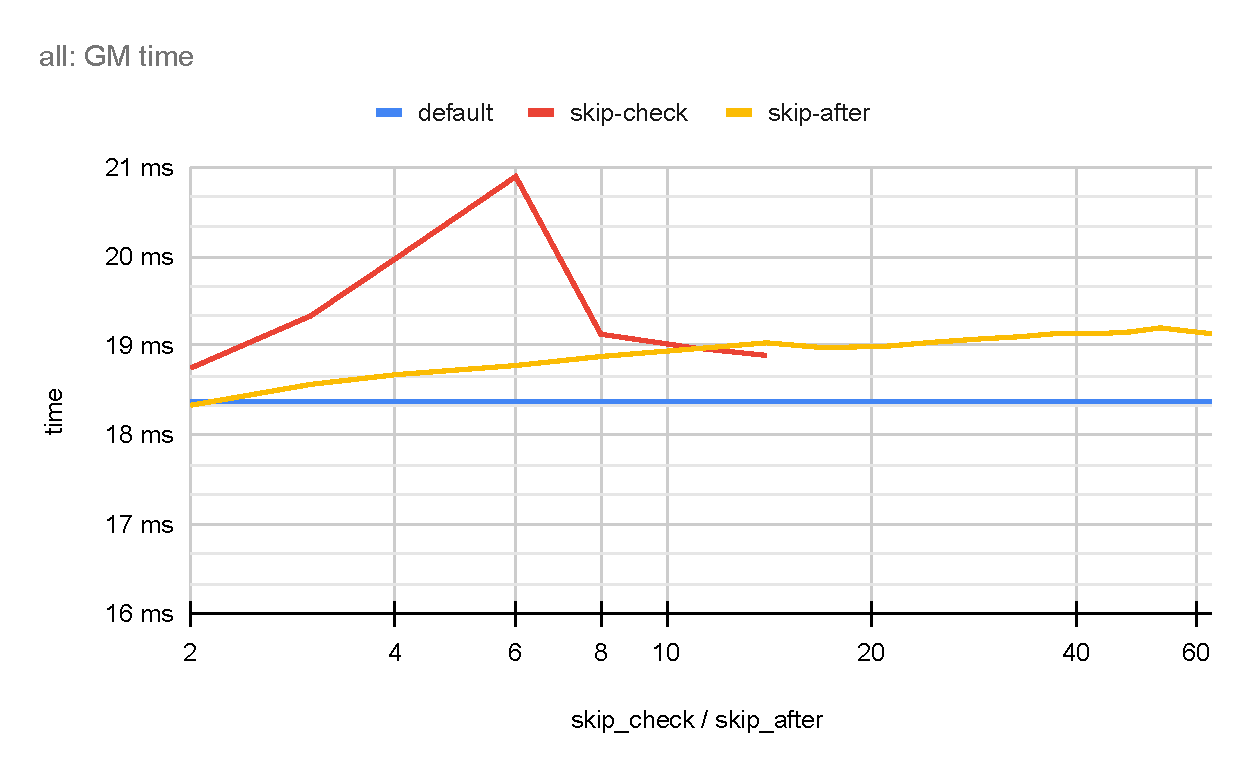
\includegraphics[width=0.48\textwidth]{out/pr-cuda-opt-d-time-gm.pdf}
    \label{fig:pr-cuda-opt-d-time-gm}
  }

  \caption{\textbf{Left:} Relative time taken for switched thread/block-per-vertex CUDA-based (GPU) static PageRank computation with the following algorithmic optimizations: no optimization (default), skip all chains (skip2), and skip chains of best min. size  (skipbest). The ratio is obtained with respect to no optimization. \textbf{Right:} GM of time taken on all graphs for switched thread/block-per-vertex CUDA-based (GPU) static PageRank computation with the following algorithmic optimizations: no optimization (none), skip converged vertices with recheck every X turns (skip-check), and skip converged vertices after X turns  (skip-after). This is relative to no optimization, with skip-check ranging from 2 to 16, and skip-check ranging from 2 to 64 (separately). Each of this is done on 5 web graphs, 4 social networks, 4 collaboration networks, and 4 road networks.}
  \label{fig:pr-cuda-opt-cd}
\end{figure*}



We then present two parallel algorithms for updating the PageRank values of vertices in a dynamic graph. Our techniques require the recomputation of the PageRank of only the vertices affected by the insertion/deletion of a batch of edges. One algorithm named \levelwisePR{}, as shown in Algorithm \ref{alg:pr-levelwise}, computes updated ranks of vertices in topological order of affected SCCs, avoiding unnecessary recomputation of SCCs that are dependent upon ranks of vertices in other SCCs which have not yet converged. We start by recomputing the PageRanks of vertices in the SCCs grouped by levels in the block-graph of the updated graph. PageRank computation is then performed on each affected level in sequential order from the topmost unprocessed level until convergence. This is repeated until all affected SCCs have been processed. The other algorithm named \monolithicPR{}, as shown in Algorithm \ref{alg:pr-monolithic}, computes updated ranks of vertices in one go, but groups vertices by SCCs and partitions them by in-degree, to obtain a better work-balance on the GPU. We first identify all the affected SCCs of updated graph. PageRank computation is then performed on all affected SCCs in every iteration, until all affected vertices appear to have converged (based on given tolerance).

\vspace{2em}
\begin{algorithm}[!hbtp]
\caption{Algorithm for computing \emph{dynamic Levelwise PageRank}. Here, $F$ is the previous snapshot of the temporal graph, $G$ is the current snapshot, and $prev$ is the initial estimate of pr (usually it is the \emph{adjusted} previous pr of vertices).}
\label{alg:pr-levelwise}
\begin{algorithmic}
\Function{dynamicLevelwisePR}{$\vars{F}, \vars{G}, \vars{prev}$}
  \State $SWITCH\_DEG \gets 64$ \Comment{indegree}
  \State $SCCs \gets affectedSCCs(F, G)$
  \State $mergeByLevel(SCCs, G)$
  \If{$GPU$}
    \State $partitionByIndeg(SCCs, G, SWITCH\_DEG)$
  \EndIf
  \Return{$\textsc{levelwiseLoop}(G, SCCs, prev)$}
\EndFunction

\Statex

\Function{levelwiseLoop}{$\vars{G}, \vars{SCCs}, \vars{prev}$}
  \State $pr \gets prev$
  \ForAll{$SCC \in SCCs$}
    \State $pr \gets \textsc{monolithicLoop}(G, [SCC], pr)$ \\  \Comment{see Algorithm \ref{alg:pr-static}}
  \EndFor
  \Return{$pr$}
\EndFunction
\end{algorithmic}
\end{algorithm}
\vspace{1em}
\vspace{2em}
\begin{algorithm}[!hbtp]
\caption{Algorithm for computing \emph{dynamic Monolithic PageRank}. Here, $F$ is the previous snapshot of the temporal graph, $G$ is the current snapshot, and $prev$ is the initial estimate of ranks (usually it is the \emph{adjusted} previous ranks of vertices).}
\label{alg:pr-monolithic}
\begin{algorithmic}
\Function{dynamicMonolithicPR}{$\vars{F}, \vars{G}, \vars{prev}$}
  \State $MIN\_WORK \gets 10^7$ \Comment{vertices}
  \State $SWITCH\_DEG \gets 64$ \Comment{indegree}
  \State $SCCs \gets affectedSCCs(F, G)$
  \If{$GPU$}
    \State $mergeMiniSCCs(SCCs, G, MIN\_WORK)$
    \State $partitionByIndeg(SCCs, G, SWITCH\_DEG)$
  \EndIf
  \Return $\textsc{monolithicLoop}(G, SCCs, prev)$ \\  \Comment{see Algorithm \ref{alg:pr-static}}
\EndFunction
\end{algorithmic}
\end{algorithm}
\vspace{1em}


Both algorithms accept the previous and current snapshot of a graph as input, along with the current (initial) ranks of the vertices. SCCs of both graph snapshots are obtained using Kosaraju's algorithm and compared, in order to obtain a list of changed SCCs. From each SCC, depth-first search (DFS) is performed in order to obtain a list of affected SCCs. We use the Compressed Sparse Row (CSR) representation of graphs for PageRank computation in order to have good memory locality. Vertices are reordered as part of preprocessing step, and computed ranks are un-reordered as part of post-processing step.

We achieve good device utilization and load balance across threads in our GPU implementation as follows. As the degree of vertices may be varying widely, we follow the general practice of choosing a thread or block of threads per vertex for calculating ranks. In order to achieve this, vertices in each SCC with an in-degree $64$ (see $SWITCH\_DEG$ in Algorithm \ref{alg:pr-monolithic}) or below are considered to be the thread-per-vertex partition where a CUDA kernel assigns the work of calculating the rank for each vertex to a single thread (belonging to a block of $512$ threads). For vertices with in-degree greater than  $64$, a CUDA kernel assigns the work of calculating the ranks of each such vertex to a block of threads (consisting of $256$ threads). We observe that grouping vertices by SCCs, and processing each SCC with a thread-per-vertex and a block-per-vertex CUDA kernel after partitioning yields better performance. Hence, this is the approach taken here. However, small affected SCCs are combined together until they satisfy a minimum work requirement of 10 million vertices (see $MIN\_WORK$ in Algorithm \ref{alg:pr-monolithic}). We do this in order to reduce the number of kernel calls. Further details of the implementation is given in our code repository \footnote{Code for this work, https://github.com/puzzlef/pagerank-multi-monolithic-vs-levelwise}.

We first compare the performance of \monolithicPR{} and \levelwisePR{} with state-of-the-art approaches. In particular, we compare our multicore implementations with the plain STIC-D algorithm (static Levelwise) \cite{pr-sticd16}, which is a static algorithm in the sense that they perform a full recomputation on the new graph. We compare our GPU implementations with the naive dynamic version of nvGraph library implementation of PageRank on a GPU \cite{pr-nvgraph}, a simplified dynamic algorithm which does not skip processing of unaffected vertices (nvGraph does not provide any parameter to control the number of vertices to be processed). We experiment with batch sizes of 500, 1000, 2000, 5000, and 10000 edges. The results of this experiment on both the CPU and the GPU is shown in Figure \ref{fig:pr-mono-vs-levl-time}. As can be noted from these figures, on the CPU, \monolithicPR{} and \levelwisePR{} achieve an average speedup of 6.1\x and 8.6\x respectively, over the STIC-D algorithm. On the GPU, \monolithicPR{} and \levelwisePR{} achieve an average speedup of 9.8\x and 9.3\x respectively, over the PageRank algorithm from the nvGraph library. We observe that \levelwisePR{} performs better on the CPU compared to \monolithicPR{}. \levelwisePR{} is computationally more efficient because it processes SCCs in topological order, avoiding unnecessary recomputation of SCCs that are dependent upon ranks of vertices in other SCCs which have not yet converged. We also observe that \monolithicPR{}{} performs better on the GPU compared to \levelwisePR{}. This is likely due to the presence of levels with insufficient work to keep the GPU busy.

We also compare the performance of our algorithms with HyPR \cite{pr-giri20}, a state-of-the-art dynamic PageRank algorithm that only recomputes ranks of affected vertices in the graph. The algorithm from HyPR runs in heterogeneous mode and utilizes both the CPU and the GPU simultaneously. To keep our comparison fair, we modify the source code of HyPR to exclusively run either on a CPU or a GPU. We run all the algorithms with a similar set of batches as above. As seen in Figure \ref{fig:pr-mono-vs-levl-time}, we observe a mean speedup of {4.2\x} and {5.8\x} for algorithms \monolithicPR{} and \levelwisePR{} respectively on the CPU, over a pure CPU implementation of HyPR. On the GPU, we observe a mean speedup of {1.9\x} and {1.8\x} for \monolithicPR{} and \levelwisePR{} respectively, over a pure GPU implementation of HyPR. The speedups can be attributed to grouping of vertices by SCCs and partitioning by in-degree in case of \monolithicPR{}, and due to the processing of affected SCCs in topological ordering in case of \levelwisePR{}.

We then contrast the performance of a batched update to a series of single edge updates (cumulative). We observe that a batch update of 5000 edges offer a speedup of 4066\x and 2998\x respectively for the monolithic and levelwise approaches on the CPU, and a speedup of 1712\x and 2324\x respectively on the GPU, as shown in Figure \ref{fig:pr-mono-vs-levl-batch}.

We observe that \levelwisePR{} is a suitable approach for CPUs. However on a GPU, smaller levels/components could be combined and processed at a time in order to help improve GPU usage efficiency as \monolithicPR suggests.
On graphs with a single SCC, the performance of the levelwise approach is noted to be almost indistinguishable from the monolithic approach. This is because a single SCC implies a single level in the block-graph for Levelwise approach to process, making its behavior is identical to that of monolithic.

\begin{figure*}[!hbtp]
  \centering

  \subfloat{
    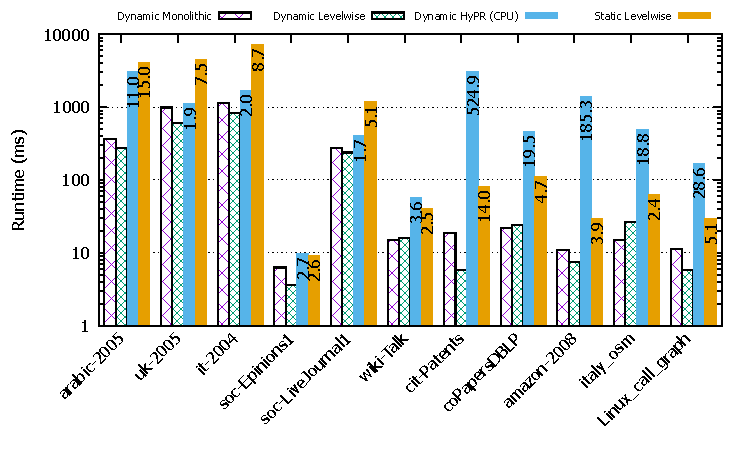
\includegraphics[width=0.48\textwidth]{out/pr-mono-vs-levl-omp-time.pdf}
    \label{fig:pr-mono-vs-levl-omp-time}
  }
  \subfloat{
    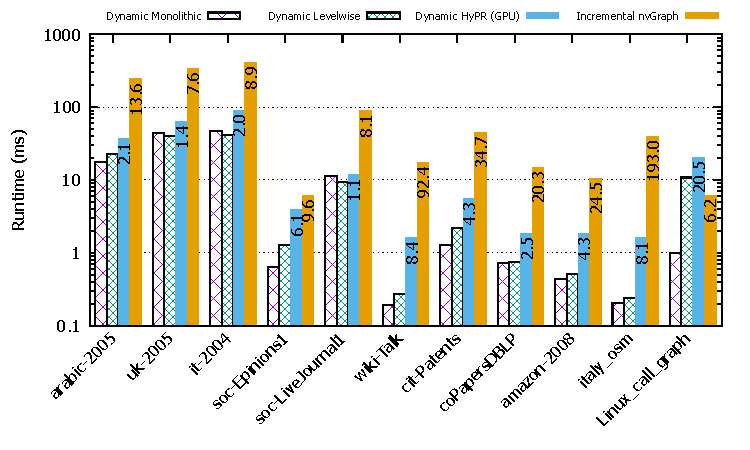
\includegraphics[width=0.48\textwidth]{out/pr-mono-vs-levl-cuda-time.pdf}
    \label{fig:pr-mono-vs-levl-cuda-time}
  }

  \caption{Time taken for PageRank computation with  \monolithicPR{} and \levelwisePR{} for various batch sizes on the CPU (shown on the left) and the GPU (shown on the right). Batch sizes of 500, 1000, 2000, 5000, and 10000 are used. Time taken with \emph{pure CPU implementation of HyPR} and \emph{plain STIC-D PageRank (static Levelwise)} on the CPU, and speedup of \levelwisePR{} over the two approaches (labeled on top of the respective bars) is also included for comparison. Time taken with \emph{pure GPU implementation of HyPR} and \emph{incremental nvGraph PageRank} on the GPU, and speedup of \monolithicPR{} over the two approaches is included as well.}
  \label{fig:pr-mono-vs-levl-time}
\end{figure*}

\begin{figure*}[!hbtp]
  \centering

  \subfloat{
    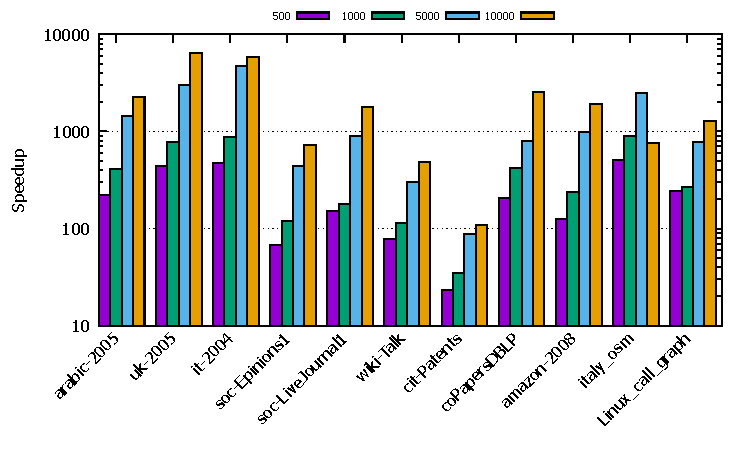
\includegraphics[width=0.48\textwidth]{out/pr-levl-omp-batch.pdf}
    \label{fig:pr-levl-omp-batch}
  }
  \subfloat{
    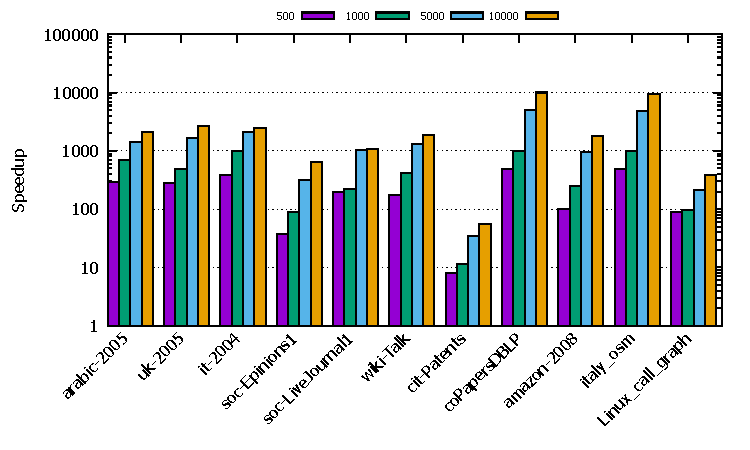
\includegraphics[width=0.48\textwidth]{out/pr-mono-cuda-batch.pdf}
    \label{fig:pr-mono-cuda-batch}
  }

  \caption{Speedup of batched \levelwisePR{} algorithm with respect to cumulative single-edge updates with the same approach on the CPU is shown on the left. Speedup of batched \monolithicPR{} algorithm with respect to cumulative single-edge updates with the same approach on the GPU is shown on the right. Batch sizes of 500, 1000, 5000, and 10000 are shown.}
  \label{fig:pr-mono-vs-levl-batch}
\end{figure*}





% We then extend the levelwise strategy of PageRank computation in the STIC-D paper to perform dynamic PageRank on the CPU as well as the GPU. We compare it to our previous monolithic CPU/GPU implementations, along with other state-of-the art implementations, such as nvGraph and HyPR. We experiment with batch sizes of 500, 1000, 2000, 5000, and 10000 edges.
% On the CPU, the monolithic and levelwise approaches achieve an average speedup of 6.1\x and 8.6\x respectively, over the STIC-D algorithm \cite{pr-sticd16}. On the GPU, an average speedup of 9.8\x and 9.3\x respectively is achieved over the PageRank algorithm from the nvGraph library. We observe a mean speedup of 4.2\x and 5.8\x respectively on the CPU, over a pure CPU implementation of HyPR \cite{hipc19}. On the GPU, we observe a mean speedup of 1.9\x and 1.8\x respectively, over a pure GPU implementation of HyPR, as shown in figure \ref{fig:pr-mono-vs-levl-time}.
